%MIT License
%
%Copyright (c) 2020 Arne Meier
%
%Permission is hereby granted, free of charge, to any person obtaining a copy
%of this software and associated documentation files (the "Software"), to deal
%in the Software without restriction, including without limitation the rights
%to use, copy, modify, merge, publish, distribute, sublicense, and/or sell
%copies of the Software, and to permit persons to whom the Software is
%furnished to do so, subject to the following conditions:
%
%The above copyright notice and this permission notice shall be included in all
%copies or substantial portions of the Software.
%
%THE SOFTWARE IS PROVIDED "AS IS", WITHOUT WARRANTY OF ANY KIND, EXPRESS OR
%IMPLIED, INCLUDING BUT NOT LIMITED TO THE WARRANTIES OF MERCHANTABILITY,
%FITNESS FOR A PARTICULAR PURPOSE AND NONINFRINGEMENT. IN NO EVENT SHALL THE
%AUTHORS OR COPYRIGHT HOLDERS BE LIABLE FOR ANY CLAIM, DAMAGES OR OTHER
%LIABILITY, WHETHER IN AN ACTION OF CONTRACT, TORT OR OTHERWISE, ARISING FROM,
%OUT OF OR IN CONNECTION WITH THE SOFTWARE OR THE USE OR OTHER DEALINGS IN THE
%SOFTWARE.
\documentclass{standalone}
\usepackage{tikz}
\usepackage[utf8]{inputenc}
\usetikzlibrary{decorations.text,arrows}


\begin{document}
	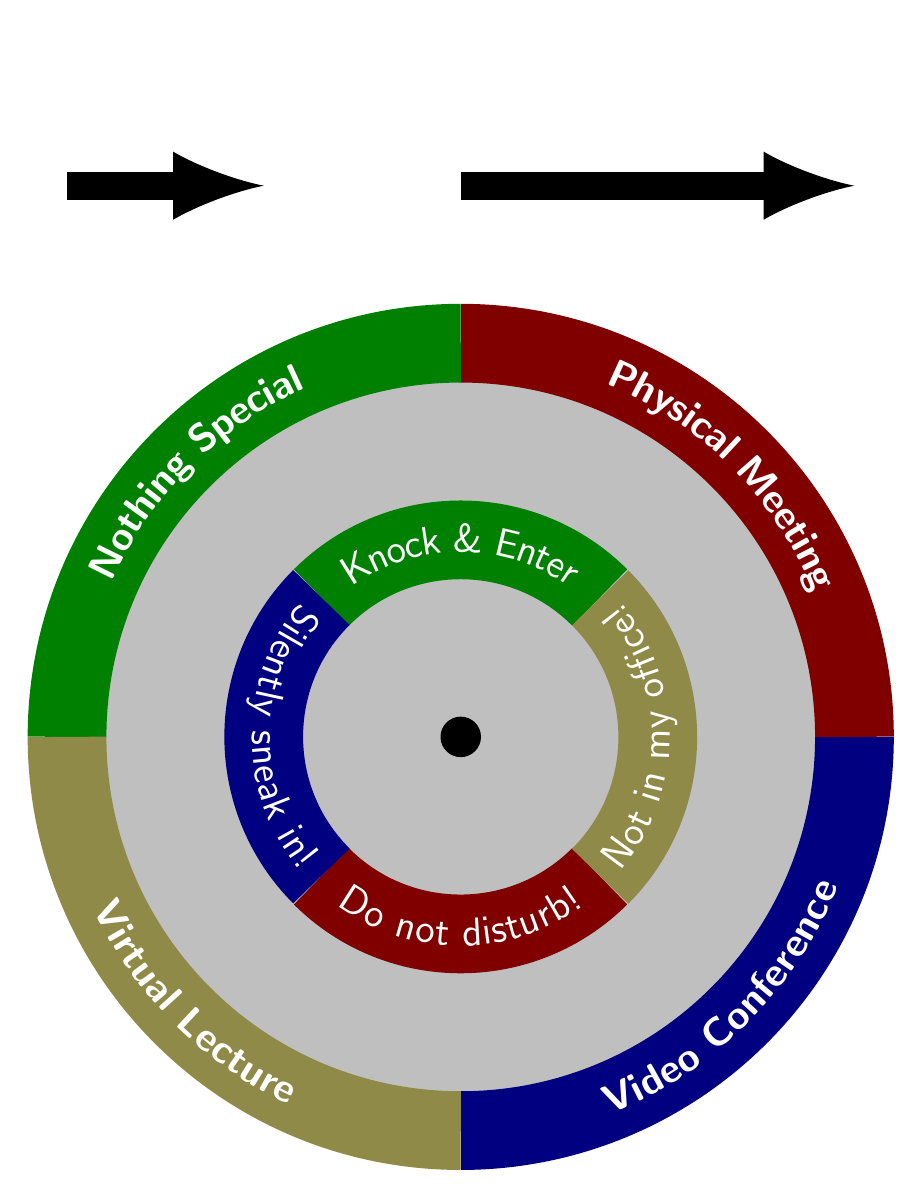
\begin{tikzpicture}
		\filldraw[lightgray] (0,0) circle (5cm);

		\filldraw[] (0,0) circle (.25cm);
		
		\path[draw=blue!50!black, line width=1cm,
			  postaction={decorate,
			  			  decoration={text effects along path, 
			  			  			  text={\ Video Conference\ }, 
			  			  			  text align=center, 
			  			  			  text effects/.cd, 
			  			  			  text along path, 
			  			  			  every character/.style={yshift=-1ex,
			  			  			  						  fill=blue!50!black}
			  			  			 },
			  			  font=\sffamily\Large\bfseries\color{white}}] (0,-5) arc [start angle=270, end angle=360, radius=5cm];
		\path[draw=red!50!black, line width=1cm,
			  postaction={decorate,
			  			  decoration={text effects along path, 
			  			  			  text={\ Physical Meeting\ }, 
			  			  			  text align=center, 
			  			  			  text effects/.cd, 
			  			  			  text along path, 
			  			  			  every character/.style={yshift=-1ex,
			  			  			  						  fill=red!50!black}
			  			  			 },
			  			  font=\sffamily\Large\bfseries\color{white}}] (0,5) arc [start angle=90, end angle=0, radius=5cm];
		\path[draw=green!50!black, line width=1cm,
			  postaction={decorate,
			  			  decoration={text effects along path, 
			  			  			  text={\ Nothing Special\ }, 
			  			  			  text align=center, 
			  			  			  text effects/.cd, 
			  			  			  text along path, 
			  			  			  every character/.style={yshift=-1ex,
			  			  			  						  fill=green!50!black}
			  			  			 },
			  			  font=\sffamily\Large\bfseries\color{white}}] (-5,0) arc [start angle=180, end angle=90, radius=5cm];
		\path[draw=yellow!50!black, line width=1cm,
			  postaction={decorate,
			  			  decoration={text effects along path, 
			  			  			  text={\ Virtual Lecture\ }, 
			  			  			  text align=center, 
			  			  			  text effects/.cd, 
			  			  			  text along path, 
			  			  			  every character/.style={yshift=-1ex,
			  			  			  						  fill=yellow!50!black}
			  			  			 },
			  			  font=\sffamily\Large\bfseries\color{white}}] (-5,0) arc [start angle=180, end angle=270, radius=5cm];
	
		\path[draw=green!50!black, line width=1cm,
			  postaction={decorate,
			  			  decoration={text effects along path, 
			  			  			  text={\ Knock \& Enter\ }, 
			  			  			  text align=center, 
			  			  			  text effects/.cd, 
			  			  			  text along path, 
			  			  			  every character/.style={yshift=-1ex,
			  			  			  						  fill=green!50!black}
			  			  			 },
			  			  font=\sffamily\Large\color{white}}] (-1.77,1.77) arc [start angle=135, end angle=45, radius=2.5cm];
		\path[draw=red!50!black, line width=1cm,
			  postaction={decorate,
			  			  decoration={text effects along path, 
			  			  			  text={\ Do not disturb!\ }, 
			  			  			  text align=center, 
			  			  			  text effects/.cd, 
			  			  			  text along path, 
			  			  			  every character/.style={yshift=-1ex,
			  			  			  						  fill=red!50!black}
			  			  			 },
			  			  font=\sffamily\Large\color{white}}] (-1.77,-1.77) arc [start angle=225, end angle=315, radius=2.5cm];

		\path[draw=blue!50!black, line width=1cm,
			  postaction={decorate,
			  			  decoration={text effects along path, 
			  			  			  text={\ Silently sneak in!\ }, 
			  			  			  text align=center, 
			  			  			  text effects/.cd, 
			  			  			  text along path, 
			  			  			  every character/.style={yshift=-1ex,
			  			  			  						  fill=blue!50!black}
			  			  			 },
			  			  font=\sffamily\Large\color{white}}] (-1.77,1.77) arc [start angle=135, end angle=225, radius=2.5cm];
		\path[draw=yellow!50!black, line width=1cm,
			  postaction={decorate,
			  			  decoration={text effects along path, 
			  			  			  text={\ Not in my office!\ }, 
			  			  			  text align=center, 
			  			  			  text effects/.cd, 
			  			  			  text along path, 
			  			  			  every character/.style={yshift=-1ex,
			  			  			  						  fill=yellow!50!black}
			  			  			 },
			  			  font=\sffamily\Large\color{white}}] (1.77,-1.77) arc [start angle=315, end angle=405, radius=2.5cm];

		\path[-latex,line width=10pt] (0,7) edge (5,7);
		
		\path[-latex,line width=10pt] (-5,7) edge (-2.5,7);
		
		\path[white] (0,9) edge (1,9);

	\end{tikzpicture}
\end{document}